% Caltech x SAIR Mathathon 2026, Problem 07: team report.
% Self-contained: no external files. Build: pdflatex report.tex (run twice).
\documentclass[11pt,letterpaper]{article}
\usepackage[T1]{fontenc}
\usepackage{lmodern,microtype}
\usepackage[margin=25mm]{geometry}
\usepackage{amsmath,amssymb,amsthm,mathtools}
\usepackage{booktabs,array,tabularx,xcolor,tikz}
\usetikzlibrary{arrows.meta,calc,decorations.pathreplacing}
\usepackage{enumitem}
\usepackage[hidelinks]{hyperref}
\usepackage{url}

\definecolor{Hc}{HTML}{C4532F}
\definecolor{Pc}{HTML}{4F7AA3}
\definecolor{lat}{HTML}{D8D4CB}
\definecolor{warn}{HTML}{C9771F}
\definecolor{itemA}{HTML}{0F6F73}
\definecolor{itemB}{HTML}{D99A1E}
\definecolor{itemC}{HTML}{7A4B9E}

\setlist{itemsep=2pt,topsep=4pt}
\setlength{\parskip}{3pt}
\setlength{\emergencystretch}{3em}
\newtheorem{theorem}{Theorem}
\newtheorem{lemma}[theorem]{Lemma}
\newtheorem{corollary}[theorem]{Corollary}
\newtheorem{claim}[theorem]{Claim}
\theoremstyle{definition}
\newtheorem{definition}[theorem]{Definition}
\theoremstyle{remark}
\newtheorem{remark}[theorem]{Remark}

\newcommand{\Hh}{\mathtt{H}}
\newcommand{\Pp}{\mathtt{P}}
\newcommand{\lean}[1]{\texttt{#1}}
\newcommand{\Z}{\mathbb{Z}}
\newcommand{\prob}[1]{\textup{\textsc{#1}}}
% Folder of the diamond-lattice Lean project in the repository (set once here).
\newcommand{\tetrapath}{lean/tetrahedral}

\begin{document}

% ================================================================ TITLE BLOCK
% Names, affiliations, the repository link and the commit hash appear ONLY here (submission rules).
\begin{center}
  {\LARGE\bfseries HP Protein Folding is NP-Complete:\\[2pt]
  a Simpler Reduction, and Lean Proofs\\[2pt] on the Cubic and Diamond Lattices\par}
  \vspace{8pt}
  {\large Team G\'en.EntityBI \;\textperiodcentered\; Caltech $\times$ SAIR Mathathon 2026, Problem 07\par}
  \vspace{8pt}
  Antonio Acuaviva\textsuperscript{1} \quad
  Pablo Acuaviva\textsuperscript{2} \quad
  Felix Schwarzfischer\textsuperscript{3}\par
  \vspace{4pt}
  {\small
  \textsuperscript{1}\,Lancaster University \quad
  \textsuperscript{2}\,University of Bern \quad
  \textsuperscript{3}\,University of M\"unster\par}
  \vspace{6pt}
  {\small
  Repository (website; Lean projects in \texttt{lean/cubic}, \texttt{lean/cooklevin},
  \texttt{lean/shelf} and \texttt{\tetrapath}):
  \url{https://github.com/caltech-mathathon-hp/caltech-mathathon-hp.github.io}\\
  Commit holding the Lean projects and the supplementary material:\\
  \texttt{f71cf8efdad993785f266ae74c266f1c21003d26}\\
  (this report and the slides were added in the commit submitted on the platform)\\
  Website: \url{https://caltech-mathathon-hp.github.io/}\par}
\end{center}

\begin{abstract}
\noindent
Berger and Leighton proved in 1998 that HP protein folding on the cubic lattice is NP-complete, by
a reduction from bin packing that is widely regarded as hard to check. We give a new reduction from
3-Partition in which all bins lie on a single edge of the forced cube: two straight crossings pin a
train of separators, and a short lemma about occupied exterior neighbours forces every gap to hold
exactly $B$ sites. This removes the padding items, the wall forcing and the switchboard routing of
the original, and we prove both directions in full. We also audited the original proof, making a
delicate face-confinement step explicit and correcting a connector bound and several smaller slips,
none of which affects the theorem. Using Lean~4 and mathlib, we checked the theorem with no
hypotheses: a Lean proof of the Cook--Levin theorem on mathlib's Turing machines, together with the
reduction chain, gives NP-completeness of both folding problems, once through a variant of our
one-edge reduction and once through a face-strip reduction. Finally we turned to a lattice that
the original proof does not reach, the four-neighbour diamond lattice, where neither the cube lemma
nor the surface gadgets exist. There we prove a new extremal lemma, whose optimal shape is an
octahedron, and a reduction from exact bin packing with separators confined by tethers to ordered windows along an edge,
and we checked in Lean, again with no hypotheses, that HP folding on the diamond lattice is
NP-complete; we know of no earlier hardness proof for the ordinary single-chain HP model on this
lattice. All Lean results were checked
with version 4.24.0, not the 4.35.0 release the competition asks for. A public website explains the
cubic proofs interactively. Section~\ref{sec:ai} describes our use of AI tools.
\end{abstract}

% ================================================================ 1
\section{Introduction}\label{sec:intro}

\subsection{The problem and the known proof}

Dill's hydrophobic--hydrophilic model~\cite{Dill85} abstracts a protein as a word over the alphabet
$\{\Hh,\Pp\}$ of hydrophobic and polar residues. A fold places the letters on distinct sites of a
lattice, with consecutive letters on adjacent sites, and its score counts the pairs of $\Hh$'s on
adjacent sites. The decision problem \prob{HP String-Fold} asks whether a given word has a fold in
$\Z^3$ whose score reaches a given threshold. Membership in NP is straightforward, since a fold is a
certificate of polynomial size; the substance of the theorem is hardness.

Berger and Leighton~\cite{BL98} proved that \prob{HP String-Fold} on $\Z^3$ is NP-complete, and in
the same year Crescenzi et al.~\cite{CGPPY98} proved the square-lattice version by an unrelated
reduction from Hamiltonian path. Berger and Leighton reduce from a form of bin packing. From an
instance they build a string with $n^3$ letters $\Hh$ and set the threshold to the number of contacts
of $n^3$ sites filling a cube, a target that is attained only when the $\Hh$'s fill an
$n\times n\times n$ cube; such a fold exists exactly when the bin-packing instance is feasible. The
$\Pp$'s are what make this work: in a cube-filling fold they all lie outside the cube, and by choosing
where they sit in the string one turns the cube into a jigsaw in which almost every piece has a
single possible position. The only freedom left is which bin each item enters.

The construction has a reputation for being hard to verify. Demaine omits the hardness proofs from
his MIT lecture on the HP model because of their complexity~\cite[transcript, p.~3]{Demaine12}, and
Istrail and Lam's survey describes them as ``quite involved''~\cite{IL09}. The problem statement of
this competition asks for exactly what is missing: ideally a formalised proof in Lean, and
alternatively a simplification of the construction.

\subsection{What is unsatisfying about the original proof}

Most of the difficulty sits in three places, each hard for a different reason. The bins are
two-dimensional: they are strips on a face, cut out by wall ribbons, and the proof must show that
every wall runs straight across the face. This requires a global argument about interacting ribbons,
including a delicate face-confinement step that a footnote of the paper treats too briefly. The source problem is general
bin packing, whose items of arbitrary size require padding items and plugs, and each of these adds
gadgets and cases. Finally, the direction from a packing to a fold joins the pieces by exterior
linkers routed through a ``switchboard'', and two of its routing lemmas are justified mainly by
figures. These features create substantial checking and formalisation obligations. Our reduction
replaces the interacting wall ribbons by intervals on one edge and gives coordinate routes for every
linker. Extending the approach to another lattice still requires an appropriate extremal shape and
new confinement gadgets, which Section~\ref{sec:new} supplies for the diamond lattice.

Most of this report concerns the cubic lattice. Our work on the square-lattice proof is partial and
is not claimed (Section~\ref{sec:site}).

\subsection{Contributions}

\begin{enumerate}[label=(\arabic*)]
  \item \emph{An audit of the original proof} (Section~\ref{sec:audit}). We wrote out every step and
    compared it with the paper. We correct a connector bound and several smaller slips, and make the
    face-confinement and routing arguments explicit.
  \item \emph{A simpler reduction} (Section~\ref{sec:edge}). We reduce 3-Partition to perfect folding
    with all bins on one edge of the cube, prove both directions, and supplement the proof with
    finite coordinate checks.
  \item \emph{A machine-checked proof} (Section~\ref{sec:lean}). Lean~4 checks, with no hypotheses,
    that both folding problems on $\Z^3$ are NP-complete. The development includes a proof of the
    Cook--Levin theorem on mathlib's Turing machines and two reductions from packing to perfect
    folding, one of them a variant of our one-edge construction.
  \item \emph{A new lattice} (Section~\ref{sec:new}). We prove that HP folding on the diamond lattice
    is NP-complete, and Lean~4 checks the theorem with no hypotheses. The proof needs a new extremal
    lemma, in which an octahedron replaces the cube, and new gadgets. We also investigated the
    face-centred cubic lattice, without reaching a hardness proof.
  \item \emph{A website and a talk} (Section~\ref{sec:site}) that explain both cubic proofs.
\end{enumerate}

\subsection{What is new and what is inherited}

To our knowledge the following are new; we make no priority claim beyond the roughly sixty papers
we reviewed, which are listed with notes on the website.
\begin{itemize}
  \item \emph{The one-edge mechanism.} Bins are gaps on one edge of the cube, a separator train is
    pinned by two straight crossings, and the \emph{gap lemma} bounds each gap by the length of the
    exterior connector, using the fact that the exterior neighbours of edge sites are already taken
    by their own $\Pp$'s. This replaces wall forcing and switchboard routing, and it works for exact
    packing with even sizes, not only for 3-Partition (Remark~\ref{rem:exact}).
  \item \emph{A machine-checked HP hardness proof, with no assumptions.} We found no earlier
    machine-checked hardness proof for the HP model in any proof assistant. Our development proves
    Cook--Levin with mathlib's finite \lean{TM2} machines and supplies it to both folding reductions;
    we make no priority claim for the Cook--Levin formalisation itself (Section~\ref{sec:lean}).
  \item \emph{NP-completeness on the diamond lattice}, through an octahedral extremal lemma and
    separators confined by tethers to ordered windows along an edge, checked in Lean. In the literature we reviewed, and
    in a further web search, we found no hardness proof for the HP model on this lattice.
  \item \emph{The audit findings} of Section~\ref{sec:audit}.
\end{itemize}
Several ingredients are inherited and credited where they are used: the HP model~\cite{Dill85}; the
cube-filling strategy, the $E$/$F$ block words and the cube frame of Berger and
Leighton~\cite{BL98}; the Loomis--Whitney inequality~\cite{LW49}; and the strong NP-completeness of
3-Partition~\cite{GJ79}. Some simplifications were found earlier during the event, in intermediate
versions of our own proof; Section~\ref{sec:edge} says which.

\subsection{Work done during the event}

All the work reported here was done during the 40 hours of the event, from 8~p.m.\ on
November~13 to noon on November~15 (Pacific Time): the audit, every version of the new reduction
and its checking programs, the Lean projects including their statement files and the proof of
Cook--Levin, the diamond-lattice proof and its formalisation, the work on the face-centred cubic
lattice, the website and the slides. Before the event we only chose
which problem to work on. The published literature we use is cited.

% ================================================================ 2
\section{Model and statements}\label{sec:model}

Throughout, $n$ denotes a positive integer, and for an integer $L\ge0$ we write $[0,L]^3$ for the set
of integer lattice sites with all coordinates in $\{0,\dots,L\}$.

\begin{definition}
A \emph{word} is $S=s_1\cdots s_N\in\{\Hh,\Pp\}^N$. A \emph{fold} of $S$ is an injective map
$f:\{1,\dots,N\}\to\Z^3$ with $\|f(i+1)-f(i)\|_1=1$ for $i<N$. Its \emph{bond score} $R(f)$ is the
number of unordered pairs $\{i,j\}$ with $s_i=s_j=\Hh$ and $\|f(i)-f(j)\|_1=1$; pairs that are
consecutive in $S$ are included.
\end{definition}

We follow Berger and Leighton in counting all adjacent $\Hh$--$\Hh$ pairs, and our talk does the
same: it calls these pairs contacts and writes the energy of a fold as $E(f)=-R(f)$, so the
decision problem asks for a fold with $E(f)\le -m$. Other authors, and the front page of our
website, count only the pairs that are not consecutive in $S$. The two scores differ by the number
$b(S)$ of factors $\Hh\Hh$ in $S$, which depends on $S$ alone, so the two conventions give the same
decision problem after a shift of the threshold. The talk illustrates the energy with three folds
of $\Hh\Pp\Hh\Hh\Hh\Hh\Pp\Hh$, a word with $b(S)=3$: the straight fold and two folds with $2$ and $4$
further contacts, of energies $-3$, $-5$ and $-7$. It also shows cube-filling folds of $\Hh^8$ and
$(\Pp\Hh\Hh\Pp)^4$, each with the $12$ bonds of a $2\times2\times2$ cube, hence $E=-12$.

\begin{definition}
\prob{HP String-Fold} asks, for a word $S$ and an integer $m$, whether $S$ has a fold with
$R(f)\ge m$. \prob{Perfect HP String-Fold} asks, for a word $S$ with exactly $n^3$ letters $\Hh$,
whether $S$ has a fold whose $\Hh$'s occupy exactly a translate of $[0,n-1]^3$; such a fold is called
\emph{perfect}.
\end{definition}

The link between the two problems is an extremal property of the cube, which is Fact~3.1 of the
paper. For a finite set $V\subset\Z^3$ let $e(V)$ be the number of lattice edges with both ends in
$V$.

\begin{theorem}[Berger--Leighton, Fact 3.1]\label{thm:cube}
If $V\subset\Z^3$ is finite and $|V|=n^3$, then $e(V)\le 3n^2(n-1)$, with equality if and only if $V$
is a translate of $[0,n-1]^3$.
\end{theorem}

\begin{proof}
Let $N=|V|$, and let $f_{xy}$, $g_{xz}$, $h_{yz}\in\{0,1\}$ indicate the three coordinate projections
of $V$, with sizes $a=\sum f_{xy}$, $b=\sum g_{xz}$, $c=\sum h_{yz}$. Put $G_x=\sum_z g_{xz}$ and
$H_y=\sum_z h_{yz}$. Two applications of the Cauchy--Schwarz inequality give the discrete
Loomis--Whitney inequality~\cite{LW49}:
\[
N\le\sum_{x,y,z}f_{xy}g_{xz}h_{yz}\le\sum_{x,y}f_{xy}\sqrt{G_xH_y}
\le\Bigl(a\sum_{x,y}f_{xy}G_xH_y\Bigr)^{1/2}\le\Bigl(a\sum_xG_x\sum_yH_y\Bigr)^{1/2}=\sqrt{abc}.
\]
A line parallel to a coordinate axis that meets $V$ in $k\ge1$ sites contains at most $k-1$ edges
of $V$, with equality exactly when those sites form an interval. There are $c$, $b$ and $a$ such
lines in the three directions, so the arithmetic--geometric mean inequality gives
\[
e(V)\le 3N-(a+b+c)\le 3N-3(abc)^{1/3}\le 3N-3N^{2/3},
\]
which equals $3n^2(n-1)$ for $N=n^3$. Suppose now that equality holds throughout. Then
$a=b=c=n^2$ and $N^2=abc$, so every inequality in the first chain is an equality. Equality in the last
step forces $f_{xy}=1$ whenever $G_x>0$ and $H_y>0$. Equality in the Cauchy--Schwarz step over $z$
forces the $0/1$ vectors $(g_{xz})_z$ and $(h_{yz})_z$ to be proportional, hence equal, for all such
pairs, so they share one support $Z$. Equality in the first step then gives $V=X\times Y\times Z$,
where $X$ and $Y$ are the active first and second coordinates. This alone does not give a cube: the
set $\{0,2\}^3$ satisfies Loomis--Whitney with equality. Equality in the line count supplies the
missing condition, since it forces every line section to be an interval, so $X$, $Y$ and $Z$ are
intervals, each of size $n$. Conversely the cube $[0,n-1]^3$ spans exactly $3n^2(n-1)$ edges.
\end{proof}

The paper invokes the inequality as ``a classic result'' without a citation and states the
uniqueness without the interval condition. Since the bond score of a fold is exactly $e(V)$ for the
set $V$ of its $\Hh$-sites, Theorem~\ref{thm:cube} gives the paper's Theorem~3.2.

\begin{corollary}[Berger--Leighton, Theorem 3.2]\label{cor:threshold}
A word with exactly $n^3$ letters $\Hh$ has a perfect fold if and only if it has a fold with bond
score at least $3n^2(n-1)$. Hence \prob{Perfect HP String-Fold} is the special case of
\prob{HP String-Fold} with threshold $3n^2(n-1)$, and it suffices to prove the perfect problem
NP-hard.
\end{corollary}

\paragraph{Local rules in a perfect fold.}
Fix a perfect fold and translate it so that its $\Hh$'s fill $C=[0,L]^3$ with $L=n-1$. Every $\Pp$
then lies outside $C$. The corners and edge sites of $C$ form its \emph{skeleton}, and the
skeleton together with the face sites forms its \emph{surface}. Three rules follow, which are
Facts~3.9--3.11 of the paper.
\begin{enumerate}[label=(\alph*)]
  \item An $\Hh$ adjacent in $S$ to a $\Pp$ has a neighbour outside $C$, so it lies on the surface.
  \item An $\Hh$ flanked in $S$ by two $\Pp$'s needs two distinct neighbours outside $C$, so it lies
    on the skeleton.
  \item In a factor $\Hh\Pp\Pp\Hh$ the two $\Hh$'s are adjacent. Their distance is odd and at most
    three, and distance three would make the three-step backbone a lattice geodesic, which stays in
    the bounding box of its end points and hence inside $C$, where no $\Pp$ can be.
\end{enumerate}
The paper justifies (c) by noting that two of the three steps are orthogonal to the surface, which
covers face sites only; the geodesic argument above covers edges and corners as well. We use the
blocks
\[
E_t=(\Pp\Hh\Pp)^t,\qquad F_t=(\Pp\Hh\Hh\Pp)^{t/2}\quad(t\text{ even}),
\]
which are also Berger and Leighton's. By (a)--(c), in a perfect fold the $\Hh$'s of $E_t$ form a
simple path of $t$ skeleton sites and those of $F_t$ a simple path of $t$ surface sites.

% ================================================================ 3
\section{The original proof and our audit}\label{sec:audit}

\paragraph{Outline.}
Berger and Leighton reduce from a modified bin packing in which the sizes $a_1,\dots,a_k$ are positive
and even, there are $K$ bins of capacity $B$, the bins must be filled exactly ($\sum a_i=KB$), and the
numbers are bounded by a polynomial in the input size. Their string consists of a frame of $E$ and
$F$ blocks, one long run of $\Hh$'s for the interior, wall ribbons, padding items and plugs, and one
$F$-ribbon per item, all joined by long runs of $\Pp$'s. In a perfect fold the frame saturates the
skeleton and five faces. On the sixth face the wall ribbons run straight across and cut the face
into strips, which serve as the bins, and each item ribbon fills part of one strip. The converse
direction folds the frame explicitly and routes all linkers through the exterior by six routing
lemmas.

In the paper's notation (its Figure~3), with item sizes $s(u)$, put $q=2\max(K,\lceil
B^{1/3}\rceil)$ for the number of strips, $n=q(2q+1)+2$, $m=n-2$, $T=(2q-1)m$ and $c=52$. With the
blocks $E_t$, $F_t$ of Section~\ref{sec:model}, the string is
\[
S_{K,B}=A\,W\,R\,\bigl(\Pp^{cn}F_{T-B}\bigr)^{q}\bigl(\Pp^{cn}F_B\bigr)^{q-K}\prod_u\bigl(\Pp^{cn}F_{s(u)}\bigr),
\]
where $A=E_{9n-10}\,F_{m^2}\,E_m\,\Pp^4(F_{m^2}\Pp^7)^3\,F_{m^2-2}\,\Pp\Hh^{m^3+2}\Pp^{8+q}$ is the frame
and the core, $W=\bigl(E_q\,F_m\,E_{2q+1}\,\Pp^4F_m\,E_q\,\Pp^{2q}\bigr)^q$ gives the walls, and
$R=\Pp\Hh(\Pp^{2q+6}\Hh)^{q-1}\Pp$ is a spaced rod. The factors $F_{T-B}$ are the paddings, the
factors $F_B$ the plugs, and the last product the items.

\paragraph{Audit.}
We wrote out every step and compared it with the RECOMB proceedings text (pp.~30--39); the website
presents the result as fifteen cards, each ending with a note. The substantive findings are these.
\begin{itemize}
  \item \emph{Footnote 7 (forming the bins, p.~38).} After each long rod the string has six $\Pp$'s,
    not two, before the next wall, so rule (c) does not apply. The footnote observes, correctly,
    that the rods' $\Pp$'s occupy every site $(0,j,-1)$ (each rod $\Hh$ uses both of its exterior
    neighbours), and then asserts that the face site $(1,b,0)$ next to the rod is the only non-edge
    face site reachable with six $\Pp$'s. Restricted to the front face this is right, but the
    footnote does not say why the next wall lies on the front face at all, and without that its
    conclusion fails: avoiding only the obstacles the footnote names, the route
    $(-1,b,0),(-2,b,0),(-3,b,0),(-3,b,1),(-2,b,1),(-1,b,1)$ reaches the interior site $(0,b,1)$ of
    the left face. (This route is a counterexample to the stated reasoning, not a fold of the
    reduction.) The missing confinement holds because the wall lies in one face and ends next to the
    opposite rail, while its first $\Hh$ is within seven steps of $(0,b,0)$, so that face must be
    the front face. If this $\Hh$ is
    $w=(i,j,0)$, the occupancy of the exterior sites forces the fifth connector $\Pp$ to be
    $(i,j,-2)$, whose distance $i+3+|j-b|$ from the first connector $\Pp$ at $(-1,b,0)$ is at most four;
    hence $i=1$ and $j=b$, and the six $\Pp$'s follow the route
    $(-1,b,0),(-1,b,-1),(-1,b,-2),(0,b,-2),(1,b,-2),(1,b,-1)$.
  \item \emph{A bound off by two (p.~38).} The paper uses $2q+6<n$ when a connector must reach from
    one free edge to another. The $\Hh$-to-$\Hh$ walk has $2q+7$ steps and the two edges are at least
    $n-1$ apart, so the condition needed is $2q+8<n$. It holds because $q\ge4$.
  \item \emph{Parity of $B$.} The plugs $(\Pp\Hh\Hh\Pp)^{B/2}$ need $B$ even, which the paper does not
    state. Nothing is lost, since every set of even items has an even total, so odd $B$ gives a
    no-instance.
  \item \emph{The source problem.} The paper asserts without proof that its modified bin packing is
    strongly NP-complete. This follows from the strong NP-completeness of 3-Partition~\cite{GJ79}: a
    3-Partition instance is an exact bin-packing instance, and doubling all numbers makes every size
    even without changing the answer. In Lean we prove it from SAT instead (Section~\ref{sec:lean}).
  \item \emph{The cube lemma and the local rules} need the interval condition and the edge-and-corner
    argument given in Section~\ref{sec:model}. The paper also uses, without stating them, two facts
    about its string on pp.~37--38: the lone $\Hh$'s fill the skeleton while the ribbons fill the face
    sites, and every exterior site adjacent to the cube holds a $\Pp$, except one site next to each
    corner.
  \item \emph{Smaller slips.} ``Since $q+1$ is odd'' should refer to $2q+1$, and ``$q-k$'' should
    be $q-K$. In Lemma~3.8 the terminal first coordinate should be $10h-7$, as in its proof; the grid
    dimension remains $10h-6$. Lemma~3.3 is justified by its figure, and Lemma~3.5 by a brief routing
    description supported by Figure~10; we supply explicit coordinate paths for both. The first
    linker starts at the spaced rod, which the text does not mention.
\end{itemize}
None of these affects the theorem, and we claim no counterexample to it.

% ================================================================ 4
\section{A simpler reduction: all bins on one edge}\label{sec:edge}

\subsection{Idea}
Instead of strips on a face, our bins are intervals on one edge of the cube, the \emph{packing
rail}. Items become rods $E_{a_i}$ on that edge, and long separators $E_g$ cut it into gaps. Only two
crossings of the working face are needed, and their sole purpose is to pin the two ends of the
separator train. A distance lemma about occupied exterior neighbours shows that each gap holds at
most $B$ sites, a count shows that the gaps hold $qB$ sites together, and so each gap holds exactly
$B$. Whatever remains of the working face is filled by a single rectangular snake.
Figure~\ref{fig:face} shows the working face schematically.

\begin{figure}[ht]
\centering
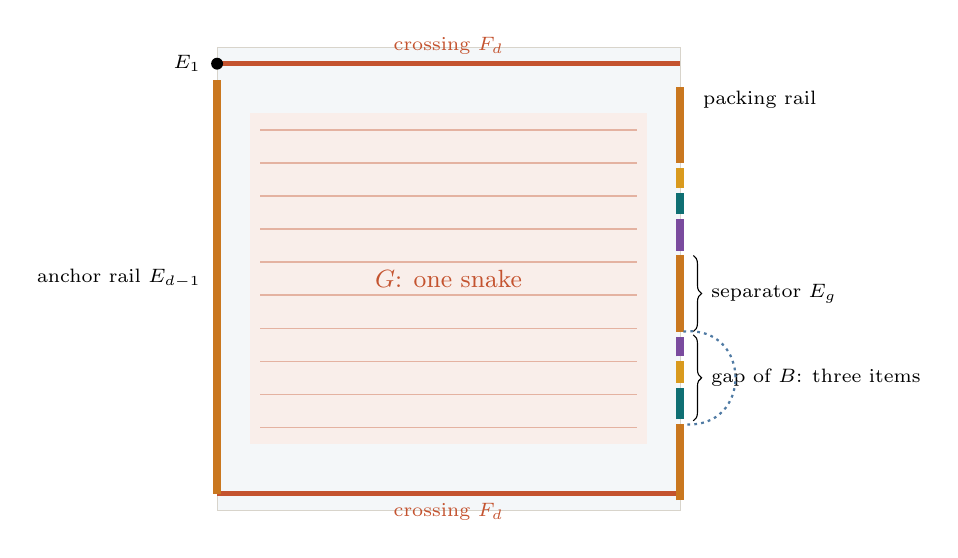
\begin{tikzpicture}[scale=0.42]
  \def\L{14}
  \fill[Pc!6] (0,0) rectangle (\L,\L);
  \draw[lat] (0,0) rectangle (\L,\L);
  \fill[Hc!10] (1,2) rectangle (13,12);
  \foreach \y in {2.5,3.5,...,11.5} \draw[Hc!45,line width=0.5pt] (1.3,\y)--(12.7,\y);
  \node[font=\small,Hc] at (7,7) {$G$: one snake};
  \draw[Hc,line width=2pt] (0,13.5)--(\L,13.5);
  \draw[Hc,line width=2pt] (0,0.5)--(\L,0.5);
  \node[font=\scriptsize,Hc,above] at (7,13.5) {crossing $F_d$};
  \node[font=\scriptsize,Hc,below] at (7,0.5) {crossing $F_d$};
  \draw[warn,line width=3pt] (0,0.5)--(0,13);
  \fill[black] (0,13.5) circle (0.18);
  \node[font=\scriptsize,left] at (-0.2,7) {anchor rail $E_{d-1}$};
  \node[font=\scriptsize,left] at (-0.2,13.5) {$E_1$};
  \foreach \a/\b in {0.3/2.6,5.4/7.7,10.5/12.8}{\draw[warn,line width=3pt] (\L,\a)--(\L,\b);}
  \draw[itemA,line width=3pt] (\L,2.75)--(\L,3.7);
  \draw[itemB,line width=3pt] (\L,3.85)--(\L,4.5);
  \draw[itemC,line width=3pt] (\L,4.65)--(\L,5.25);
  \draw[itemC,line width=3pt] (\L,7.85)--(\L,8.8);
  \draw[itemA,line width=3pt] (\L,8.95)--(\L,9.6);
  \draw[itemB,line width=3pt] (\L,9.75)--(\L,10.35);
  \draw[decorate,decoration={brace,amplitude=3pt}] (\L+0.4,5.3)--(\L+0.4,2.7)
    node[midway,right=3pt,font=\scriptsize] {gap of $B$: three items};
  \draw[decorate,decoration={brace,amplitude=3pt}] (\L+0.4,7.7)--(\L+0.4,5.4)
    node[midway,right=3pt,font=\scriptsize] {separator $E_g$};
  \node[font=\scriptsize,right] at (\L+0.4,12.4) {packing rail};
  \draw[Pc,line width=0.8pt,dash pattern=on 1pt off 1.5pt] (\L+0.1,5.4)..controls (\L+2.2,5.6) and (\L+2.2,2.4)..(\L+0.1,2.6);
\end{tikzpicture}
\caption{Schematic view of the working face in a perfect fold of the one-edge string. The anchor
rail is the left edge and the packing rail the right edge. Two straight rows, the crossings $F_d$,
join the rails at the top and bottom and pin both ends of the train of $q+1$ separators on the
packing rail. Between consecutive separators lie the $q$ gaps, each holding three item rods. The
dotted curve stands for a separator connector $\Pp^{B+2}$, which runs outside the cube. The snake $G$
fills the rest of the face.}
\label{fig:face}
\end{figure}

\subsection{The construction}

\begin{theorem}\label{thm:edge}
From an instance of unary 3-Partition one can construct in polynomial time a word $S$ with exactly
$n^3$ letters $\Hh$ such that the following are equivalent:
\begin{enumerate}[label=(\roman*)]
  \item the instance has a 3-partition;
  \item $S$ has a perfect fold;
  \item $S$ has a fold with bond score at least $3n^2(n-1)$.
\end{enumerate}
Moreover $|S|=n^3+O(n^2)$ and $n$ is linear in the unary input length. Consequently
\prob{Perfect HP String-Fold} and \prob{HP String-Fold} on $\Z^3$ are NP-complete.
\end{theorem}

\paragraph{Parameters.}
A valid instance has $q\ge1$ and consists of $3q$ positive integers $a_i$ and a bound $B$ with $\sum a_i=qB$ and
$B/4<a_i<B/2$, written in unary; since 3-Partition is strongly NP-complete~\cite{GJ79}, it remains
NP-complete in this form. An integer strictly between $B/4$ and $B/2$ exists only if $B\ge3$. We
double every $a_i$ and $B$, which preserves the feasible partitions and gives $B\ge6$, with $B$ and all
$a_i$ even and $a_i\ge2$. Instances with $q=1$ and malformed inputs are handled separately below, so
assume $q\ge2$ and set
\begin{equation}\label{eq:params}
  g=B+6,\qquad d=(q+1)g+qB,\qquad n=d+2,\qquad L=d+1,\qquad K=8n.
\end{equation}
Then $d$ is even, $d\ge 48$ and $B+5<g<L$. The cube is $C=[0,L]^3$; each of its edges has $d$
non-corner sites, and the skeleton has $12d+8$ sites.

\paragraph{The word.}
With $E_t$ and $F_t$ as in Section~\ref{sec:model}, define
\[
\begin{aligned}
  A&=E_{9d+8}\,F_{d^2}\,E_d, & D&=\Pp\,\Hh^{d^3+2}\,\Pp\,F_{d^2-2},\\
  W&=E_1\,F_d\,E_g\,(\Pp^{B+2}E_g)^q\,F_d\,E_{d-1}, & G&=F_{d(d-2)},
\end{aligned}
\]
and
\begin{equation}\label{eq:word}
  S \;=\; A\,\Pp^K\,(F_{d^2}\Pp^K)^3\,D\,\Pp^K\,W\,\Pp^K\,G\,\prod_{i=1}^{3q}\bigl(\Pp^K E_{a_i}\bigr).
\end{equation}
Every parameter, every linker length and every letter of $S$ depends on the instance alone. The $E$
blocks contain $(10d+8)+(d+(q+1)g)+qB=12d+8$ letters $\Hh$, the $F$ blocks (including the two
crossings and $G$) contain $6d^2-2$, and the bulk run contributes $d^3+2$, for a total of
$(d+2)^3=n^3$.

\subsection{A perfect fold gives a 3-partition}

Fix a perfect fold and translate it so that its $\Hh$'s fill $C$.

\paragraph{Step 1: the skeleton is saturated.}
The $\Hh$'s flanked by two $\Pp$'s are exactly the $12d+8$ $\Hh$'s of $E$ blocks, since every $\Hh$ of
an $F$ block has an $\Hh$ neighbour in $S$ and the bulk run has length at least two. By rule (b) they
all lie on the skeleton, which has exactly $12d+8$ sites, so they fill it and no other $\Hh$ lies on
it. By rule (c), every $E$ or $F$ block, and every adjacent $E$--$F$ join, compresses to a simple
$\Hh$-path. An $F$ path consists of surface sites off the skeleton, so it lies in the interior of a
single face.

\paragraph{Step 2: three free edges and two rails.}
A simple path on the skeleton through $t$ corners consists of at most $t+1$ edge segments, each
with at most $d$ non-corner sites, so it has at most $t+(t+1)d\le 9d+8$ sites. The block $E_{9d+8}$
attains this bound, so it passes through all eight corners and nine complete edges. Nine segments of
non-corner sites separated by eight corners require both end points to be non-corner sites, so
each corner is interior to the path and uses two of its three edges; the three
remaining edges are therefore pairwise disjoint, and their non-corner sites form three separate
components of $d$ sites each. The final $E_d$ of $A$ fills one of them. The other two, the
\emph{rails}, are left for $W$ and the items.

\paragraph{Step 3: a single working face.}
The four blocks $F_{d^2}$ fill four face interiors, and $F_{d^2-2}$ fills a fifth face up to two sites.
Each of the two crossings $F_d$ and the block $G$ has more than two $\Hh$'s and is a connected path in
one face interior, so all three lie in the sixth face, which we call the \emph{working face}.

\paragraph{Step 4: the crossings anchor the train.}
Every $E$ block outside $A$ is a skeleton path avoiding $A$, hence an interval of one rail. The block
$E_{d-1}$ fills all but one site of a rail, the \emph{anchor rail}. Separators $E_g$ and items have at
least two $\Hh$'s each and so cannot use that last site; they all lie on the other rail, the
\emph{packing rail}, and $E_1$ fills the remaining anchor site. The first crossing joins $E_1$ to the
first separator and the second joins the last separator to $E_{d-1}$, so both crossings join the two
rails, which are therefore opposite sides of the working face. Choose face coordinates with the
anchor rail at $x=0$, the packing rail at $x=L$, and $1\le y\le d$ along the rails. Oriented from the
anchor rail to the packing rail, a crossing together with its two rail end points has $d+1=L$ steps
and increases $x$ by $L$, so every step increases $x$: each crossing is a straight row, and its two
rail end points have the same $y$. Since the anchor occupies $[1,d-1]$ or $[2,d]$, the two ends of
the separator train are at $y$-distance $1$ or $d-1$.

\paragraph{Step 5: the separators come in order.}
Each separator is an interval of $g$ sites. The terminal $\Hh$ of one separator and the initial $\Hh$
of the next are joined by $B+5$ backbone steps: the $B+2$ inserted $\Pp$'s and one $\Pp$ from each $E$
block. Suppose a separator is traversed in increasing $y$ and ends at $b$. An interval of length $g$
to its left has both end points at distance at least $g$ from $b$, and so does an interval to its
right that is entered at its far end. Since $B+5<g$, both are impossible, so the next separator lies
to the right and is traversed in increasing $y$. By induction all $q+1$ separators lie in backbone
order with a common orientation, and the train's two ends are at distance at least $(q+1)g-1>1$.
Hence they are at distance $d-1$: the train runs from one end of the packing rail to the other, with exactly
$q$ gaps between consecutive separators.

\begin{lemma}[Gap lemma]\label{lem:gap}
If two consecutive separators have $r$ rail sites between them, then $r\le B$.
\end{lemma}

\begin{proof}
There is nothing to prove for $r=0$, so let $r\ge1$; the two $\Hh$'s facing each other across the
gap are then at distance $r+1$. Every site between them holds an $\Hh$ of an $E$ block. Such an $\Hh$,
lying on an edge but not at a corner, has exactly two neighbours outside $C$, and its two flanking
$\Pp$'s occupy both. None of these $\Pp$'s belongs to the connector between the two separators, so the
connector avoids every exterior neighbour of every intervening $\Hh$. A connector path outside $C$
needs at least two steps transverse to the edge, one to leave it and one to return. A path of length
at most $(r+1)+2$ would therefore move monotonically along the edge with exactly one step out and one
step back, and all intermediate positions along the edge would be visited at one fixed outward
normal, that is, at an occupied exterior neighbour. So such a path does not exist. Since the lattice
is bipartite, the length of a path has the parity of the distance between its end points, and the
connector needs at least $(r+1)+4=r+5$ steps. It has exactly $B+5$, so $r\le B$.
\end{proof}

\begin{figure}[ht]
\centering
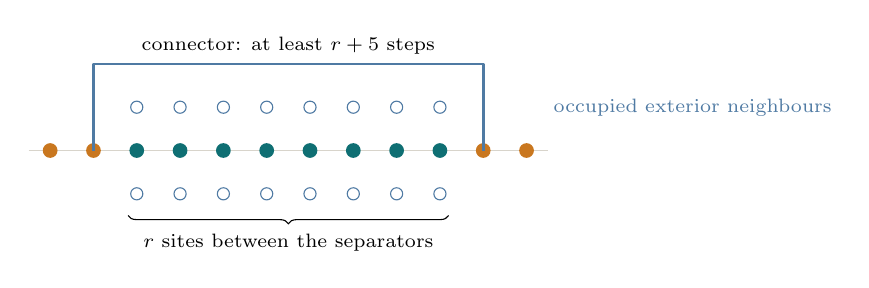
\begin{tikzpicture}[x=0.55cm,y=0.55cm]
  \draw[lat,line width=0.6pt] (-1.5,0)--(10.5,0);
  \foreach \x in {-1,0} \fill[warn] (\x,0) circle (0.17);
  \foreach \x in {9,10} \fill[warn] (\x,0) circle (0.17);
  \foreach \x in {1,...,8} {\fill[itemA] (\x,0) circle (0.17);
     \draw[Pc] (\x,1) circle (0.14); \draw[Pc] (\x,-1) circle (0.14);}
  \node[font=\scriptsize,Pc,right] at (10.4,1) {occupied exterior neighbours};
  \draw[Pc,line width=1pt,line join=round] (0,0)--(0,2)--(9,2)--(9,0);
  \draw[decorate,decoration={brace,amplitude=3pt,mirror}] (0.8,-1.5)--(8.2,-1.5)
     node[midway,below=3pt,font=\scriptsize] {$r$ sites between the separators};
  \node[font=\scriptsize,above] at (4.5,2) {connector: at least $r+5$ steps};
\end{tikzpicture}
\caption{Schematic cross-section for the gap lemma. The packing rail runs horizontally; the two
separator ends are on the left and right, and the $r$ sites between them hold item $\Hh$'s. Each of
these has its two exterior neighbours (open circles, drawn above and below) occupied by its own
$\Pp$'s, so the connector must step out to depth two and come back, which takes at least $r+5$
steps.}
\label{fig:gap}
\end{figure}

\paragraph{Step 6: reading off the partition.}
The packing rail has $d$ sites and the separators occupy $(q+1)g$ of them, so the $q$ gaps hold
$d-(q+1)g=qB$ sites together. By Lemma~\ref{lem:gap} each holds at most $B$, so each holds exactly
$B$. Every item is an interval of the packing rail and cannot cross a separator, so it lies in a
single gap. The items have $qB$ $\Hh$'s and fill all the gaps, so the sizes of the items in each gap
add up to $B$, and the bounds $B/4<a_i<B/2$ force exactly three items per gap. This is a
3-partition, which proves (ii)$\Rightarrow$(i). Since $S$ has $n^3$ letters $\Hh$,
Corollary~\ref{cor:threshold} gives (ii)$\Leftrightarrow$(iii).

\begin{remark}\label{rem:exact}
The bounds $B/4<a_i<B/2$ are used only in the last sentence of Step~6, to conclude that each gap
holds exactly three items. Without them the same argument shows that the items in each gap have
total size $B$, so the construction is equally a reduction from exact bin packing with positive even
sizes and $\sum a_i=qB$; the completeness direction below uses only $a_i\ge2$ and $k\le qB/2$ for the
number $k$ of items. The fifth instance of the supplementary computations is of this kind.
\end{remark}

\begin{remark}
The connector length $\Pp^{B+2}$ is chosen for the gap lemma. A length count that ignored the occupied
exterior neighbours would only give $r\le B+2$, which is too weak.
\end{remark}

\subsection{A 3-partition gives a perfect fold}

Assume a 3-partition is given. We first place every block, including all of its $\Pp$'s, and then
supply every linker $\Pp^K$ with exactly its length.

\paragraph{Placements.}
\emph{Snakes} traverse rows alternately forward and backward; in a box, the row snake is reversed in
alternate layers. \emph{Face words}: on a simple $\Hh$-path $h_1,\dots,h_{2t}$ in a face with outward
normal $v$, the factor $\Pp\Hh\Hh\Pp$ number $j$ is placed at $h_{2j-1}+v,\,h_{2j-1},\,h_{2j},\,h_{2j}+v$;
consecutive $\Pp\Pp$ joins are adjacent because their $\Hh$ projections are. \emph{Edge words}: an
edge site that is not a corner has two exterior neighbours (a corner has three), and the two $\Pp$'s of
each $\Hh$ of an $E$ block go to two distinct exterior neighbours of its site. On a straight edge, the
links $\Hh\Pp\Pp\Hh$ alternate between the two exterior normals; an $E$ block of even length can have
the same normal for its first and last $\Pp$, and one of odd length has different end normals. A
general simple skeleton path is lifted to its $E$ word greedily from the end: consecutive sites
have two common exterior normals, and each step is given a common normal different from the label
of the next step, starting from a prescribed final normal. Each exterior site adjacent to $C$ has a
unique neighbour in $C$, so $\Pp$'s assigned to different $\Hh$'s never collide.

\paragraph{Frame and bulk.}
We use coordinates in which $x$ runs from left to right, $y$ from bottom to top and $z$ from front
($z=0$) to back ($z=L$). The block $E_{9d+8}$ of $A$ follows the skeleton polyline
\begin{multline*}
(d,L,L)\to(0,L,L)\to(0,L,0)\to(L,L,0)\to(L,L,L)\\
\to(L,0,L)\to(L,0,0)\to(0,0,0)\to(0,0,L)\to(d,0,L),
\end{multline*}
two square perimeters joined by an edge, with $9d+8$ sites, lifted with its final $\Pp$ pointing out of
the back face. The block $F_{d^2}$ of $A$ snakes through the back face with $x$ decreasing from $d$ to
$1$ and $y$ alternating, and $A$'s final $E_d$ fills the edge $(0,y,L)$, $1\le y\le d$, with both end
$\Pp$'s pointing to the back. The two edges left free are $x=0,z=0$ (the anchor rail) and $x=L,z=0$ (the
packing rail). The left, bottom and right face interiors are filled by snakes whose $\Pp$'s point
along the outward face normals, with the following end points:
\begin{center}\small
\begin{tabular}{@{}lll@{}}
\toprule
Block & first $\Hh$ & last $\Hh$\\
\midrule
$A$ & $(d,L,L)$ & $(0,d,L)$\\
left face & $(0,1,1)$ & $(0,d,1)$\\
bottom face & $(d,0,d)$ & $(d,0,1)$\\
right face & $(L,1,d)$ & $(L,d,d)$\\
$D$ & $(d,L,1)$ & $(d-1,L,1)$\\
\bottomrule
\end{tabular}
\end{center}
The block $D$ begins with a $\Pp$ at $(d,L+1,1)$ and an $\Hh$ at $(d,L,1)$. It fills the
$d\times d\times d$ interior by a layered box snake from $(d,d,1)$ to $(d,d,d)$, reversing the layer
path in each layer, so that the evenness of $d$ puts the end point at $(d,d,d)$; it then visits an
$\Hh$ at $(d,L,d)$ and a $\Pp$ at $(d,L+1,d)$. It ends with the top-face snake from $(d,L,d)$ to
$(d,L,1)$ with its first and last sites removed, which realises $F_{d^2-2}$ from $(d-1,L,d)$ to
$(d-1,L,1)$. This places every letter of $D$ and leaves no hole in the top face.

\paragraph{The block $W$, the snake $G$ and the items.}
The separators occupy the intervals $I_j=[1+j(g+B),\;g+j(g+B)]$, $0\le j\le q$, of the packing rail
$(L,y,0)$, leaving $q$ gaps of $B$ sites each. The block $W$ starts with $E_1$ at $(0,d,0)$, with its
first $\Pp$ pointing left and its last pointing to the front. Its first $F_d$ crosses row $y=d$ from
$x=1$ to $x=d$. It then traverses the separators in decreasing $y$, starting with $I_q$, and gives
both end $\Pp$'s of every separator the front normal. Two consecutive separators whose facing
$\Hh$'s are in rows $b$ and $c=b-B-1$ are joined in front of the face by
$(L,b,-1)\to(L,b,-2)\to(L,c,-2)\to(L,c,-1)$, which has exactly $B+2$ new sites; these connectors lie
over disjoint gaps at depth two. After the last separator reaches row $1$, the second $F_d$ traverses
row $1$ from $x=d$ down to $x=1$, and $W$ ends with $E_{d-1}$ on $(0,y,0)$, $1\le y\le d-1$, with its
first $\Pp$ pointing to the front and its last pointing left. The snake $G$ fills the rectangle
$1\le x\le d$, $2\le y\le d-1$, $z=0$, starting at $(d,2,0)$ with $x$ decreasing and ending at
$(d,d-1,0)$, with front normals; together with the two crossings it fills the working face. In each
gap we place its three items in increasing $y$, in any order, with both end $\Pp$'s pointing right,
which is possible because the sizes are even. Gaps begin at odd $y$ and items have even size, so each
item starts at an odd row and ends at an even row, all item end rows are distinct, and all are at
most $d-g<d-1$. Item $\Pp$'s lie at depth one to the front or to the right, while $W$'s connectors lie
at depth two in front with $x=L$, so they do not collide.

At this point every block is placed injectively, the $\Hh$'s fill $C$, and all $\Pp$'s placed so far lie in
the first two layers outside $C$.

\paragraph{Linker length and parity.}
Colour $\Z^3$ by the parity of the coordinate sum. In the placement above, the first $\Hh$ of every
block is even and its last $\Hh$ is odd. A linker $\Pp^K$ between two blocks must therefore be realised
by an $\Hh$-to-$\Hh$ path of exactly $K+3$ edges, which is odd. The first two vertices of this path are
the preceding block's last $\Hh$ and its final $\Pp$, the last two are the next block's initial $\Pp$
and its first $\Hh$, and the remaining $K$ vertices are the inserted $\Pp$'s.

\paragraph{The corner route.}
For two ports on adjacent faces, we use local coordinates in which $u$ and $v$ are the signed
outward distances from the two faces and $t$ runs along their common edge. After exchanging the ports
if necessary, their $\Hh$'s are $p=(0,-s,t_0)$ and $q=(-r,0,t_1)$ with $0\le r,s\le L$ and $t_0>t_1$.
For a depth $h$ and a turning coordinate $T>t_0$, the route consists of the axis-parallel segments
\begin{multline}\label{eq:corner}
p\to(h,-s,t_0)\to(h,h+1,t_0)\to(h,h+1,T)\\
\to(h+1,h+1,T)\to(h+1,h+1,t_1)\to(-r,h+1,t_1)\to q.
\end{multline}
Its first and last steps leave along the outward face normals. It is simple, because the outgoing
arm and the returning track are separated in $u$, the turn lies beyond both ports in $t$, and $t_0>t_1$
keeps the returning arm off the outgoing track. All its sites other than $p$ and $q$ are outside
$C$. With $T=\max(t_0,t_1)+1$ its length is $\ell=4h+s+r+|t_0-t_1|+6$, and each increase of $T$ by one
adds two steps without affecting any of the separation properties below.

\paragraph{The seven frame linkers.}
The linkers up to item~1 join, in order, $A$ to the left face, the left face to the bottom face, the
bottom face to the right face, the right face to $D$, $D$ to $W$, $W$ to $G$, and $G$ to item~1. Linker
$j$ uses route~\eqref{eq:corner} with depth $h_j=4+2j$ and the following ports:
\begin{center}\small
\begin{tabular}{@{}cll@{}}
\toprule
$j$ & faces & common-edge coordinates of the two ports\\
\midrule
1 & back, left & $d$, $1$\\
2 & left, bottom & $1$, $d$\\
3 & bottom, right & $1$, $d$\\
4 & right, top & $d$, $1$\\
5 & top, left & $1$, $0$\\
6 & left, front & $d-1$, $2$\\
7 & front, right & $d-1$, $y_1$\\
\bottomrule
\end{tabular}
\end{center}
Here $y_1\le d-g$ is the first row of item~1, and the two coordinates in each row are distinct. We
check that the routes avoid the fixed blocks and each other.
\begin{enumerate}[label=(\roman*)]
  \item \emph{Stems.} The outward stems have distinct $\Hh$ projections. Every other fixed $\Pp$ at
    depth one belongs to a different $\Hh$; $W$'s depth-two connectors have $x=L$ and point to the
    front, while item stems point right and $G$'s stems have $x=d$.
  \item \emph{Earlier arms and later stems.} Every arm of a later linker has a coordinate at outward
    depth at least $h_j$, deeper than every earlier arm or stem, so an earlier arm can meet a later
    stem only on a face they share, and there they are separated explicitly. On the left face the
    first arm has $y=1$ and $z\ge1$, the next has $z=1$, and $W$'s ports have $z=0$, with $W$'s first
    port leaving toward the top from $y=d$ and so missing its final port at $y=d-1$. On the bottom face
    the earlier arm has $z=d$ and the later port $z=1$. On the right face both full-face arms have
    $z=d$ and the item ports have $z=0$, and the earlier arm leaves $y=1$ toward $0$, missing the later
    full-face port at $y=d$. On the top face the earlier arm moves from $x=d$ toward $L$, while the later
    port has $x=d-1$. On the front face the earlier arm has $y=2$ and the later port $y=d-1$.
  \item \emph{Outer parts.} The two tracks and the turn of route $j$ form its outer part, whose two
    assigned outward coordinates both lie in the band $\{h_j,h_j+1\}$. An outer part cannot meet a
    stem, since a stem leaves $C$ in only one coordinate. Any two outer parts share an assigned
    coordinate axis; on that axis their outward signs are opposite or their depth bands are disjoint,
    so they do not intersect. For an outer part and an arm with the same pair of assigned axes,
    separation follows from their depth bands or outward signs. For an outer part and an arm with
    different pairs of assigned axes, one exterior coordinate of the outer part is the arm's
    common-edge coordinate, which stays in $[0,L]$ along the arm, so they cannot meet.
\end{enumerate}
These facts give mutual disjointness for arbitrary turning coordinates $T$. All parts other than
stems have depth at least six and so miss the fixed blocks. Since $h_j\le18$ and $r,s,|t_0-t_1|\le L$,
we have $\ell_j\le 3L+78=3n+75<K+3$, and $\ell_j$ is odd because the two port parities differ.
Choosing $T=\max(t_0,t_1)+1+(K+3-\ell_j)/2$ gives exactly $K+3$ edges.

\paragraph{The item linkers.}
There are $k=3q$ items, and $k\le qB/2<d/4$ since every $a_i\ge2$. For $i=1,\dots,k-1$ we join item
$i$'s last $\Hh$ $(L,u,0)$ to item $i+1$'s first $\Hh$ $(L,v,0)$ by a rectangle in the plane $x=L+h_i$,
with $h_i=20+i$:
\begin{equation}\label{eq:item}
(L,u,0)\to(L+h_i,u,0)\to(L+h_i,u,-R_i)\to(L+h_i,v,-R_i)\to(L+h_i,v,0)\to(L,v,0).
\end{equation}
All item end rows are distinct, so every stem has its own row; an arm stays in its end row, and the
segment joining the two rows has $z<0$ and misses all stems at $z=0$. Different linkers lie in
different planes, and each rectangle is simple because $u\ne v$ and $R_i\ge1$. The seven frame routes
also miss these rectangles. Frame routes on the right face and the bottom or top have their right-face
arms at $z=d$ and their outer parts at $y<0$ or $y>L$. The front--right route to item~1 has rightward
depth at most $19$ and its front arm at $y=d-1$, whereas item routes have rightward depth at least
$21$ and rows below $d-1$; its entry stem lies in item~1's first row, which no later item linker uses.
The remaining frame routes have $x\le L$. At $R_i=1$ the length of~\eqref{eq:item} is
$2h_i+2+|u-v|\le d+2k+39<\tfrac32 d+39<K+3$, and the end rows have opposite parity, so
$R_i=(K+3-2h_i-|u-v|)/2$ is a positive integer for which the path has exactly $K+3$ edges. All
coordinates used are $O(n)$.

The blocks and linkers now spell $S$ in its original order. Every step is a lattice edge, every
residue has its own site, every $\Pp$ is outside $C$, and the $n^3$ $\Hh$'s lie in $C$ and therefore fill
it. This proves (i)$\Rightarrow$(ii).

\subsection{Size, exceptional inputs, NP membership and thresholds}
Doubling multiplies the unary input size by a constant, and $n=d+2$ is linear in it. The bulk run
has $d^3+2$ letters and everything else has $O(n^2)$ letters (there are $3q+6$ linkers of length
$O(n)$), so $|S|=n^3+O(n^2)$. A valid instance with $q=1$ is a yes-instance and is mapped to the
perfect-folding instance $(\Hh,n=1)$. A malformed input is mapped to $(\Hh^7\Pp\Hh,n=2)$, which has no
perfect fold: its $\Hh$'s occupy five positions of one parity and three of the other, while a
$2\times2\times2$ cube has four sites of each colour, and a fold maps positions of equal parity to
sites of equal colour. For the threshold problem we use the corresponding thresholds from
Corollary~\ref{cor:threshold}. Both problems are in NP. The empty word is handled directly: its
bond score is zero, and it cannot fill a cube of positive side. For a nonempty word, translate the
first residue of a fold to the origin, so that all coordinates are at most $|S|$ in absolute value, and check injectivity,
adjacency, the score and cube coverage in polynomial time. With the strong NP-completeness of
3-Partition~\cite{GJ79} this proves Theorem~\ref{thm:edge}. For the convention that excludes
consecutive $\Hh\Hh$ pairs, $S$ has $d^3+3d^2$ such pairs ($3d^2-1$ from the $F$ blocks and $d^3+1$
from the bulk run), and the threshold becomes $3n^2(n-1)-(d^3+3d^2)=2n^3-4$.

\subsection{Comparison with the original proof}

\begin{center}
\small
\begin{tabularx}{\linewidth}{@{}>{\raggedright\arraybackslash}p{0.2\linewidth}>{\raggedright\arraybackslash}X>{\raggedright\arraybackslash}X@{}}
\toprule
& Berger--Leighton (bins as face strips) & This work (bins on one edge)\\
\midrule
Source problem & modified bin packing, with padding items and plugs & 3-Partition (or exact packing
  with even sizes), no padding\\
Item gadget & $F$-ribbon filling part of a strip & rod $E_{a_i}$ on one edge\\
Crossings of the working face & wall ribbons between all strips, which must be forced straight & two
  crossings, straight by a length count\\
Bin forcing & straight walls and anchor counting & separator order, gap lemma, total length\\
Rest of the working face & strip fillings around the items & one snake $G$\\
Routing & switchboard, six routing lemmas & seven corner routes, then one rectangle per item link\\
\bottomrule
\end{tabularx}
\end{center}

On our proof boards (website and talk) the original proof has fifteen steps, three of which we rate
as hard to check, and the one-edge proof has seventeen steps, one of them hard: routing the seven
frame linkers around the corners of the cube. The new proof is not smaller in numbers, since for the
same $B$ its parameter $d$ is larger. Its gain is that the packing argument becomes one-dimensional.
The routing comparison refers to Berger and Leighton's switchboard; an intermediate face-bin version
of our own already used a single corner-routing lemma for every long linker, and the one-edge proof's
two families of routes are not simpler than that version.

\paragraph{A worked example.}
The talk shows both strings for one small instance, the items $1,1,2$ in two bins of size $2$, with
pictures of their folds from the website. For Berger and Leighton's string the sizes are doubled
(items $2,2,4$, $B=4$, $K=2$), which gives $q=4$, $n=38$, $T=252$ and linkers $\Pp^{1976}$; the
string has $54{,}872$ letters $\Hh$ and consists of the frame and core
\[
(\Pp\Hh\Pp)^{332}(\Pp\Hh\Hh\Pp)^{648}(\Pp\Hh\Pp)^{36}\Pp^{4}\bigl((\Pp\Hh\Hh\Pp)^{648}\Pp^{7}\bigr)^{3}(\Pp\Hh\Hh\Pp)^{647}\Pp\Hh^{46658}\Pp^{12},
\]
the walls and the spaced rod
$\bigl((\Pp\Hh\Pp)^{4}(\Pp\Hh\Hh\Pp)^{18}(\Pp\Hh\Pp)^{9}\Pp^{4}(\Pp\Hh\Hh\Pp)^{18}(\Pp\Hh\Pp)^{4}\Pp^{8}\bigr)^{4}\,\Pp\Hh(\Pp^{14}\Hh)^{3}\Pp$,
the paddings and plugs
$\bigl(\Pp^{1976}(\Pp\Hh\Hh\Pp)^{124}\bigr)^{4}\bigl(\Pp^{1976}(\Pp\Hh\Hh\Pp)^{2}\bigr)^{2}$, and the items
$\Pp^{1976}\Pp\Hh\Hh\Pp\;\Pp^{1976}\Pp\Hh\Hh\Pp\;\Pp^{1976}(\Pp\Hh\Hh\Pp)^{2}$. The one-edge string shown
next to it is that of the shelf variant formalised in Lean (Section~\ref{sec:lean}), not the string
\eqref{eq:word}: the sizes and $B$ are multiplied by $6$ and one full bin is added (items
$6,6,12,12$, $B=12$, $m=3$), so $n=m(B+1)+3=42$ and the string has $74{,}088$ letters $\Hh$. It
reads
\begin{multline*}
\Hh^{73600}\Pp\Pp\,\Hh(\Pp\Pp\Hh)^{367}\Pp^{176}\Hh(\Pp\Pp\Hh)^{39}\;\;
\Pp^{42}\Hh(\Pp^{18}\Hh)^{3}\Pp^{42}\Hh(\Pp\Pp\Hh)^{39}\\
\Pp^{176}\Hh(\Pp\Pp\Hh)^{5}\,\Pp^{176}\Hh(\Pp\Pp\Hh)^{5}\,\Pp^{176}\Hh(\Pp\Pp\Hh)^{11}\,\Pp^{176}\Hh(\Pp\Pp\Hh)^{11}\Pp,
\end{multline*}
in which the first group is the core and frame, the second holds the four single-$\Hh$ separators
with their two tethers $\Pp^{42}$, and the third the four items. For the construction of this
section the same instance, doubled, has $q=2$, $B=4$, $g=10$, $d=38$ and $n=40$.

\paragraph{How we arrived at it.}
The starting point was the observation that the padding items and plugs exist only to handle general
bin packing, so a special family of instances should make them unnecessary; 3-Partition, whose
items lie strictly between $B/4$ and $B/2$, turned out to be that family. We first rewrote the original
proof with 3-Partition as the source and rectangular bins on a face, which removes paddings and
plugs. We then simplified the wall forcing (fixed two-site gaps, a counting modulus larger than the
number of bins, and items too large for the two leftover surface sites), placed all item end points
on one line, and finally moved the bins onto one edge. Each stage was written up with a complete
proof and checked on explicit instances. The gap lemma and the separator train first appear in the
last stage.

\subsection{Supplementary computations}
The following computations check finite instances; the proof above does not depend on them. They
were made with a standard-library JavaScript program, written for this construction without
importing the code of our earlier constructions or their checkers, and supplied with its output as
supplementary material.
\begin{itemize}
  \item \emph{Complete folds.} For five instances the program builds the entire fold of the literal
    word $S$, including the bulk and every inserted $\Pp$, and checks every backbone step, global
    injectivity, that every $\Hh$ lies in the cube and every $\Pp$ outside, exact coverage, and both
    scores. After doubling, the instances are $(q,B)=(2,6)$, $(3,6)$, $(2,12)$ and $(2,20)$, all strict
    3-Partition instances (the last with the non-uniform sizes $6,8,6,6,6,8$), and an exact packing
    with sizes $2,4,4,2$ that is not a 3-Partition instance. The cube sides are $n=50$, $68$, $80$, $120$
    and $50$. Together the folds have 3{,}023{,}224 residues, the largest 1{,}825{,}956 residues and
    1{,}728{,}000 $\Hh$'s. All checks passed.
  \item \emph{Gap distances.} For $r=0,\dots,12$, breadth-first search in a local model of the
    exterior near the rail (the box $u\in[-2,4]$, $z\in[-4,2]$, $y\in[-4,r+5]$, with the first-layer
    exclusions used by the construction) finds shortest connectors of length $3$ for $r=0$ and $r+5$
    for $1\le r\le12$, in agreement with Lemma~\ref{lem:gap}.
  \item \emph{Separator order.} For $q\in\{2,3,4\}$ and $B\in\{2,4,6\}$, an exhaustive search places the
    $q+1$ separators one after another on a rail of $d$ sites, in any position and direction, subject
    only to the anchor condition of Step~4 and the connector bound of Lemma~\ref{lem:gap}, which is
    taken as input. In every case it finds exactly two placements, one for each end of the rail at
    which the train can start, and in both all separators share one direction, the train spans the
    rail, and every gap has exactly $B$ sites.
\end{itemize}

% ================================================================ 5
\section{Lean formalisation}\label{sec:lean}

\paragraph{Version.}
The repository's \lean{lean/} folder holds three Lean projects for the cubic lattice:
\lean{lean/cubic}, the reduction chain through a face-strip construction; \lean{lean/cooklevin}, a
proof of the Cook--Levin theorem; and \lean{lean/shelf}, which proves the final theorems through a
variant of our one-edge reduction and combines everything into hypothesis-free statements. A fourth
project, \lean{\tetrapath}, proves the diamond-lattice theorem and is described in
Section~\ref{sec:new}. The competition requires Lean and Mathlib v4.35.0. All our projects are
pinned to Lean and mathlib v4.24.0 (in \lean{lean-toolchain}, \lean{lakefile.toml} and
\lean{lake-manifest.json}); we started with this version and did not port the projects during the
event. Every statement below that
we describe as checked in Lean was checked with Lean and mathlib 4.24.0. The projects have not been
verified in the required 4.35.0 environment, and they may not build there without changes.

\subsection{What is proved}

\paragraph{Statements and definitions.}
The model, the encodings and the complexity notions are defined once, in six statement files: words,
folds and the bond score, \prob{HP String-Fold} and \prob{Perfect HP String-Fold} on $\Z^3$, their
binary encodings, and polynomial-time decidability, NP, Karp reductions, NP-hardness and
NP-completeness on top of mathlib's \lean{TM2} Turing machines. The pinned mathlib provides
polynomial-time machines and computable reducibility notions but no class NP~\cite{mathlib}, so the
verifier-based NP class and the polynomial-time Karp reductions used here are our own definitions,
built on its \lean{TM2} interface: a problem is in NP when a polynomial-time machine checks a certificate of polynomial
length, a Karp reduction is a function computed by a polynomial-time machine that preserves the
answer, and a problem is NP-hard when every NP problem reduces to it. The statement files were
written first and then frozen; the audit compares their SHA-256 hashes with the recorded ones, so any
later change to them would be detected. Lean checks that definitions are well-typed and that proofs
are correct, but it cannot tell whether a definition expresses the intended informal notion, so the
website shows these definitions in full for comparison with the paper. The score counts all adjacent
$\Hh\Hh$ pairs, as in Section~\ref{sec:model}. Lean's perfect-folding input type also permits side
$n=0$, at which exactly the words without $\Hh$ are accepted, the empty word among them, whereas
Section~\ref{sec:model} uses positive sides. Both hardness constructions output positive sides, so
hardness holds for either convention; references to the Lean perfect-folding declarations use
Lean's convention.

\paragraph{The Cook--Levin theorem.}
The statement that SAT is NP-hard is the proposition \lean{SAT.CookLevin}, defined as
\lean{NPHard cnfEncoding Satisfiable} for CNF formulas with binary variable indices. In
\lean{lean/cubic} the three hardness theorems take it as an explicit hypothesis \lean{hCL}, which is
not an axiom: Lean checks that the theorems follow from it. The project \lean{lean/cooklevin} proves
the proposition with no hypotheses, as \lean{SAT.CookLevinUniversal.cookLevin}, in 130 modules whose
only external dependency is mathlib. The proof uses a computation tableau. A single finite
\lean{TM2} verifier runs on the encoded pair of input and certificate for a polynomially bounded
number of steps, and local cell and window constraints describe its padded run. The resulting CNF
formula has polynomial encoded size and is satisfiable exactly when some certificate within the
prescribed bound is accepted. An explicit polynomial-time \lean{TM2} machine emits the formula, up to
a bijective renaming of variables, and a polynomial-time post-processor produces clauses of width at
most three (\lean{SAT.CookLevinUniversalWidthThree.npHard}). Cook--Levin has been mechanised in
Coq~\cite{GK21}, in Isabelle~\cite{Balbach23} and in several Lean developments; in particular,
\lean{lean-np-hardness} reports a complete proof with mathlib's finite \lean{TM2}
machines~\cite{Solresol26}, and RBarish's AI-written development uses a separate machine
model~\cite{RBarish26}. We make no priority claim for our Cook--Levin formalisation.

\paragraph{The first certificate (\lean{lean/cubic}).}
The main results are
{\small
\begin{verbatim}
theorem perfectIffThreshold_holds : PerfectIffThreshold
theorem hpStringFold_inNP :
  InNP hpEncoding (fun I : HPInstance => I.Accepts)
theorem perfectHPStringFold_inNP :
  InNP perfectEncoding (fun I : PerfectInput => PerfectHPStringFold I.1 I.2)
theorem perfectHPStringFold_NPHard     (hCL : SAT.CookLevin) : PerfectHPStringFoldNPHard
theorem perfectHPStringFold_NPComplete (hCL : SAT.CookLevin) :
  PerfectHPStringFoldNPComplete
theorem hpStringFold_NPComplete        (hCL : SAT.CookLevin) : HPStringFoldNPComplete
\end{verbatim}
}
\noindent The hardness results here carry the hypothesis \lean{hCL}; it is discharged in
\lean{lean/shelf}, as described below. The threshold equivalence and both memberships in NP are proved without hypotheses; the
memberships come with explicit polynomial-time \lean{TM2} verifiers. Hardness follows the chain
\begin{multline*}
\text{CNF}\;\to\;\text{balanced 3D matching}\;\to\;\text{positive-even unary exact packing}\\
\to\;\text{perfect cubic folding}\;\to\;\text{HP threshold folding},
\end{multline*}
in which each arrow is a Karp reduction: a map that is total on the typed instance space and handles
invalid instance fields explicitly, a proof that it preserves the answer, and a \lean{TM2} machine
with a proved polynomial running time. The machines are specified on canonical encodings of
instances; we do not assert that every malformed serialized word is rejected. The paper's appeal to
Garey and Johnson for strong NP-hardness of bin packing is thereby replaced by a proof from SAT. The
packing-to-folding step uses an alternative frame of the face-strip type (a saturated skeleton,
modular anchor counting, straight crossings with no spare steps, rectangular item strips of even
width, and routes at distinct depths). It is not a line-by-line formalisation of the paper's Figure~3
string or of its Lemmas~3.3--3.8, but both geometric directions are proved for it.

\paragraph{The second certificate (\lean{lean/shelf}).}
This project builds on an unchanged copy of the first project's library and replaces only the step
from exact packing to perfect folding, by a one-edge or ``shelf'' reduction. An instance is
normalised (all sizes and $B$ are multiplied by $6$, and if the number $m$ of bins is even, one bin and
one item of size $B$ are added) and written as a string with $n^3$ $\Hh$'s, where $n=m(B+1)+3$. One edge
of the cube, the shelf, carries $m+1$ separators, each a single $\Hh$, and two tethers hold the first
and last separators at the ends of the shelf. The shelf has $n-2=mB+(m+1)$ non-corner sites; the
$m+1$ separators occupy one site each, leaving exactly $mB$ sites for the items, so every gap is
exactly full and holds items of total size $B$. This is a variant of the construction of
Section~\ref{sec:edge}, with different gadgets: single-$\Hh$ separators and a tether lemma take the
place of long separators, two crossings and the gap lemma. The construction of
Section~\ref{sec:edge} itself is a paper proof and is not formalised in Lean as written.

The shelf project vendors the first project's library and adds the Cook--Levin files, without
editing any of them. Continuous integration checks the files listed in the manifest
\lean{vendor/cook\_levin\_files.sha256} against that manifest, both in \lean{lean/cooklevin} and in
the shelf's vendor directory. The file \lean{Shelf/NPComplete.lean} first proves the final theorems from the hypothesis
\lean{hCL}, and \lean{Shelf/Unconditional.lean} then substitutes \lean{SAT.CookLevinUniversal.cookLevin}
for it. This gives
{\small
\begin{verbatim}
theorem Shelf.Unconditional.perfectHPStringFold_NPComplete :
  PerfectHPStringFoldNPComplete
theorem Shelf.Unconditional.hpStringFold_NPComplete : HPStringFoldNPComplete
\end{verbatim}
}
\noindent with no hypotheses. The same substitution applied to the first project's chain gives the
theorems \lean{perfectHPStringFold\_NPComplete} and \lean{hpStringFold\_NPComplete} in the namespace
\lean{Shelf.Unconditional.TeamRoute}. So the NP-completeness of both
folding problems on $\Z^3$ is checked in Lean without hypotheses, by two routes that differ only in
the reduction from packing to perfect folding.

\paragraph{Declarations the report relies on.}
All names are in the namespace \lean{ProteinFolding}. The first table lists the declarations of
\lean{lean/cubic}.
\begin{center}\footnotesize
\begin{tabularx}{\linewidth}{@{}>{\raggedright\arraybackslash}p{0.47\linewidth}>{\raggedright\arraybackslash}X@{}}
\toprule
Declaration & Claim it supports, and how it differs from the claim\\
\midrule
\lean{CubicGeometry.\allowbreak positiveEdgeCount\_le\_cube},\newline
  \lean{CubicGeometry.\allowbreak positiveEdgeCount\_eq\_cube\_iff}
  & Theorem~\ref{thm:cube}, under the hypothesis $|s|=n^3$. \lean{positiveEdgeCount} counts each
  lattice edge once, in its positive coordinate direction. No additional unproved premise.\\
\lean{perfectIffThreshold\_holds} & Corollary~\ref{cor:threshold}, as an equivalence of the two
  decision problems. No hypothesis.\\
\lean{hpStringFold\_inNP}, \lean{perfectHPStringFold\_inNP} & Both problems are in NP, with binary
  input encodings. No hypothesis.\\
\lean{ThreeDimensionalMatching.\allowbreak cnfToBlockMatching\_karp} & CNF reduces to balanced 3D matching.\\
\lean{MatchingPacking.matching\_karpReduces\_modified} & 3D matching reduces to exact packing with
  even sizes in unary.\\
\lean{SATPacking.modifiedBinPackingUnary\_NPHard} & That packing problem is NP-hard. Hypothesis
  \lean{hCL}.\\
\lean{CubicPacking.packingToPerfect\_correct}, \lean{CubicPacking.packingToPerfect\_karp} & Packing
  reduces to perfect folding, through the alternative face-strip frame, not the paper's string.\\
\lean{perfect\_karpReduces\_hp} & Perfect folding reduces to threshold folding.\\
\lean{perfectHPStringFold\_NPHard}, \lean{perfectHPStringFold\_NPComplete},
  \lean{hpStringFold\_NPComplete} & Berger and Leighton's theorem. Hypothesis \lean{hCL}.\\
\bottomrule
\end{tabularx}
\end{center}

\noindent The second table lists the declarations of \lean{lean/shelf} and \lean{lean/cooklevin},
together with the statement \lean{SAT.CookLevin} from \lean{lean/cubic}.
\begin{center}\footnotesize
\begin{tabularx}{\linewidth}{@{}>{\raggedright\arraybackslash}p{0.47\linewidth}>{\raggedright\arraybackslash}X@{}}
\toprule
Declaration & Claim it supports, and how it differs from the claim\\
\midrule
\lean{Shelf.foldGivesPacking}, \lean{Shelf.packingGivesFold}, \lean{Shelf.reductionCorrect},
  \lean{Shelf.shelfKarp} & The shelf reduction is a correct polynomial-time Karp reduction. No
  hypothesis. This is the shelf variant, not the construction of Section~\ref{sec:edge}.\\
\lean{Shelf.perfectHPStringFold\_NPComplete},\newline \lean{Shelf.hpStringFold\_NPComplete} & The same
  final theorems, through the shelf reduction. Hypothesis \lean{hCL}.\\
\lean{SAT.CookLevin} & The statement that SAT is NP-hard (a proposition).\\
\lean{SAT.CookLevinUniversal.cookLevin} & Cook--Levin: SAT is NP-hard, for CNF with binary variable
  indices. No hypothesis.\\
\lean{Shelf.Unconditional.\allowbreak perfectHPStringFold\_NPComplete},\newline
  \lean{Shelf.Unconditional.\allowbreak hpStringFold\_NPComplete} & Both folding problems on $\Z^3$ are
  NP-complete, through the shelf reduction. No hypothesis.\\
\lean{Shelf.Unconditional.TeamRoute.\allowbreak perfectHPStringFold\_NPComplete},\newline
  \lean{Shelf.Unconditional.TeamRoute.\allowbreak hpStringFold\_NPComplete} & The same, through the
  face-strip reduction of the first project. No hypothesis.\\
\bottomrule
\end{tabularx}
\end{center}

\subsection{What ``checked in Lean'' means here}
We call a statement checked in Lean when (i) the project builds with the pinned toolchain; (ii) no
\lean{sorry} remains in its proof or in anything the proof uses; (iii) \lean{\#print axioms} lists only
\lean{propext}, \lean{Classical.choice} and \lean{Quot.sound}; (iv) the proof does not use
\lean{native\_decide}; and (v) the declaration, after unfolding its definitions and taking its
hypotheses into account, expresses the claim attributed to it. Conditions (i)--(iv) hold for every
declaration in the two tables, supported by the builds, the axiom reports and the source scans.
Condition (v) requires mathematical review; the tables record the correspondence and any
differences in convention. The same five conditions are what we mean for the diamond-lattice
theorem of Section~\ref{sec:new}, where condition (i) was met in our working copy by compiling the
project's modules one by one, as described there. The
first project's audit script also compares every source file with a SHA-256 manifest, searches the
code (with comments and strings removed) for forbidden constructs, and prints the axioms of the
named public declarations within its documented scope. Some imported modules are not enumerated
individually by that script; their contribution to the main results is covered by the axiom reports
of those results. Since \lean{\#print axioms} does not show hypotheses, the hypothesis \lean{hCL},
where present, appears only in the type of a theorem; the unconditional theorems have none. The
repository's workflow \lean{lean-certificates.yml} builds each of the three cubic-lattice projects and runs its
axiom checks (the full audit for \lean{lean/cubic}) on pushes to \lean{main} that change the Lean
folders; the shelf job also checks its copies of the Cook--Levin files against \lean{lean/cooklevin}.

\paragraph{Reproducing the checks.}
The diamond-lattice project has its own instructions, given in Section~\ref{sec:new} and in its
README. For the three cubic-lattice projects, with \lean{elan} installed, run in each project folder
{\small
\begin{verbatim}
lake exe cache get
lake build
\end{verbatim}
}
\noindent followed by these checks:
{\small
\begin{verbatim}
lake env lean checks/CubicHardness.lean       # in lean/cubic
pwsh -NoProfile -File checks/Verify.ps1       # in lean/cubic (full audit)
lake env lean checks/AxiomAudit.lean          # in lean/cooklevin
lake env lean checks/ShelfHardness.lean       # in lean/shelf
\end{verbatim}
}

\paragraph{Prior formal work.}
We found no earlier machine-checked hardness proof for HP folding in any proof assistant. The only
Lean library for the HP model we found~\cite{Ptyche} defines folds and bounds their contacts but
contains no hardness results.

% ================================================================ 6
\section{A new lattice: the diamond lattice}\label{sec:new}

Our cubic construction, like Berger and Leighton's, uses the extremality of the cube and gadgets
confined to its faces and edges. Neither is available off the shelf on other three-dimensional
lattices, and no hardness proof for the HP model on them was known to us. We carried the method
over to the four-neighbour diamond lattice, where it yields a complete proof that Lean checks, and
we investigated the face-centred cubic lattice, where no hardness proof was reached. For completeness of the status
table in our talk: the square and cubic lattices are settled~\cite{CGPPY98,BL98}; the survey of
Istrail and Lam lists hardness on the hexagonal lattice as open~\cite{IL09}, we know of no hardness
proof on the triangular lattice either, and we did not work on these two lattices.

\subsection{The diamond lattice}

The diamond (tetrahedral) lattice $\mathcal D$ consists of the sites $(x,y,z)\in\Z^3$ with
$x\equiv y\equiv z\pmod 2$ and $x+y+z\equiv0$ (sublattice $A$) or $3$ (sublattice $B$) modulo~$4$. With
the bond vectors $t_1=(1,1,1)$, $t_2=(1,-1,-1)$, $t_3=(-1,1,-1)$ and $t_4=(-1,-1,1)$, an $A$-site $v$
is adjacent to the four sites $v+t_k$ and a $B$-site $v$ to the four sites $v-t_k$. The graph is
$4$-regular and bipartite, with girth $6$. Words, folds and the bond score are defined as on $\Z^3$:
a fold is injective on all residues, the lattice is fixed and infinite, and all adjacent
$\Hh$--$\Hh$ pairs are counted, including consecutive ones. An instance is a word and an integer
threshold written in binary; there is no scaffold, obstacle or bounding box.

\begin{theorem}[checked in Lean~4.24.0, no hypotheses]\label{thm:diamond}
\prob{HP String-Fold} on the diamond lattice is NP-complete.
\end{theorem}

\paragraph{The octahedron.}
For $m\ge1$ put $N_m=m(4m^2-1)/3$. With $c=(0,2m-2,0)$ and, for each of the eight sign vectors
$\sigma\in\{\pm1\}^3$, $\beta(\sigma)=2m-2$ if $\sigma_1\sigma_2\sigma_3=+1$ and $\beta(\sigma)=2m-1$
otherwise, the \emph{octahedron} is
\[
\mathrm{Oct}(m)=\{v\in\mathcal D:\ \sigma\cdot(v-c)\le\beta(\sigma)\text{ for all eight }\sigma\},
\]
which has $N_m$ sites. Its eight faces come in two kinds, four ``big'' and four ``small''.

\paragraph{Structure of the proof.}
The proof follows Berger and Leighton's plan, with a new extremal lemma and new gadgets.
\begin{enumerate}[label=(\arabic*)]
  \item \emph{Extremal lemma.} A set of $N_m$ sites of $\mathcal D$ spans at most $2N_m-2m^2$ bonds,
    with equality exactly when a symmetry of the lattice maps it onto $\mathrm{Oct}(m)$ (in the
    manuscript: when it is a translate of $\mathrm{Oct}(m)$ or of its mirror image). Between each
    pair of consecutive coordinate layers the lattice bonds form zigzag chains. Each maximal run of
    occupied sites on these chains contributes two bonds leaving the set, and a composition
    inequality bounds the size of a set in terms of its total number of runs. Consequently a word with $N_m$ letters $\Hh$ has a fold with
    $2N_m-2m^2$ bonds exactly when it has a fold whose $\Hh$'s fill an octahedron. This plays the
    role of Theorem~\ref{thm:cube} and Corollary~\ref{cor:threshold}.
  \item \emph{The word}, built from exact bin packing with numbers in unary ($K$ bins of capacity
    $B$, positive sizes with total $KB$). It consists of a rigid frame laid along two edges of one
    small face of the octahedron; dimer chains of $\ell\ge1$ dimers, with word
    $(\Hh\Hh\Pp\Pp\Pp)^{\ell-1}\Hh\Hh$, placed between long $\Pp$-runs, whose dimers can only lie on
    edges of the octahedron in a fold attaining $2N_m-2m^2$ bonds; $K+1$ separators, each held by
    two long $\Pp$-runs (tethers); the items, as dimer chains of length proportional to their sizes;
    fillers; and long runs of $\Hh$'s for the interior.
  \item \emph{A fold attaining the threshold gives a packing.} In such a fold the frame is rigid
    and the dimers form a perfect matching of the remaining edge sites. Put $\Sigma_*=18K+40$ and
    $\lambda=\Sigma_*+8$; an item of size $a$ is a chain of $\lambda a$ dimers. The tethers confine
    the separators to disjoint, ordered windows on a third edge, and each gap between consecutive
    separators is filled by whole item chains. The number of dimers in a gap is a multiple of
    $\lambda$ and, by the size of the windows, differs from $\lambda B$ by less than $\lambda$, so
    it equals $\lambda B$. Thus the $K$ gaps give an exact packing of the source items. As in
    Section~\ref{sec:edge}, the bins are intervals on one edge; here tethers of bounded length and
    the scaling by $\lambda$ do the work of the two crossings and the gap lemma.
  \item \emph{A packing gives a fold attaining the threshold.} All $\Hh$'s are placed on
    $\mathrm{Oct}(m)$, the interior being covered by an explicit family of disjoint paths, and the
    $\Pp$'s are routed outside: near the surface by explicit local rules, and far away by a
    product-like scheme that realises every prescribed linker length and parity.
\end{enumerate}
Membership in NP is proved as on $\Z^3$, by a polynomial-time verifier for a fold given as a list of
directions.

\paragraph{The Lean proof.}
The formalisation is the project \lean{\tetrapath} of the repository. It reuses the
shared definitions of words, folds, the bond score, encodings and NP-completeness
(Section~\ref{sec:lean}). Its statement files (the lattice, the problem, the input encoding and the
target) were written first and are pinned by hash. The target and the theorem are
{\small
\begin{verbatim}
def HPStringFoldNPComplete : Prop :=
  NPComplete hpEncoding (fun I : HPInstance => I.Accepts)
theorem tetrahedral_hp_npComplete : HPStringFoldNPComplete
\end{verbatim}
}
\noindent in the namespace \lean{ProteinFolding.Tetrahedral}, with no hypotheses; \lean{\#print axioms}
reports only \lean{propext}, \lean{Classical.choice} and \lean{Quot.sound}. The theorem combines
membership in NP, the hardness of the source problem, which comes from our Lean proof of
Cook--Levin and the reduction chain of Section~\ref{sec:lean}, and a Karp reduction computed by a
polynomial-time \lean{TM2} machine from the packing instance alone. The declarations are listed
below. The names \lean{reduction\_sound}, \lean{reduction\_complete} and \lean{reduction\_correct}
all belong to \lean{ReductionTM2.Canonical}. The extremal and threshold declarations assume $m>0$
and the stated cardinality $N_m$, and the acyclicity statement assumes $m\ge50$; none requires an
additional unproved premise.
\begin{center}\footnotesize
\begin{tabularx}{\linewidth}{@{}>{\raggedright\arraybackslash}p{0.47\linewidth}>{\raggedright\arraybackslash}X@{}}
\toprule
Declaration (in \lean{ProteinFolding.Tetrahedral}) & Claim it supports\\
\midrule
\lean{tetrahedral\_hp\_npComplete} & Theorem~\ref{thm:diamond}.\\
\lean{hp\_inNP} & Membership in NP, with an explicit polynomial-time verifier.\\
\lean{PackingSource.\allowbreak unary\_exact\_capacity\_npHard} & Exact bin packing with numbers in
  unary is NP-hard.\\
\lean{ReductionTM2.Canonical.computable} & The reduction is computed in polynomial time.\\
\lean{ReductionTM2.Canonical.reduction\_sound},\newline \lean{reduction\_complete},
  \lean{reduction\_correct} & Steps (3) and (4): the output is accepted exactly when the packing
  instance is.\\
\lean{bondCount\_octahedral\_bound\_int},\newline
  \lean{contact\_maximizer\_iff\_\allowbreak normalizes\_to\_octahedron} & Step (1): the bound
  $2N_m-2m^2$ for folds with $N_m$ letters $\Hh$, and its equality case for sets of $N_m$ sites.\\
\lean{octahedral\_threshold\_iff\_oct\_support} & A fold reaches the threshold exactly when its
  $\Hh$'s fill an octahedron.\\
\lean{bulkFiniteGraph\_acyclic} & The path cover of the interior is acyclic for every $m\ge50$.\\
\bottomrule
\end{tabularx}
\end{center}
\noindent The import closure of the final check within this folder has 884 modules, counting the
audit module itself; the shared library and mathlib are additional dependencies.

Three points about this formalisation should be stated plainly. First, the proof contains finite
case analyses (234 reference components of the interior path cover and 1{,}920 joint certificate
rows, among others). Lean's kernel checks them by evaluation (\lean{decide} with kernel
reduction); the proof uses neither \lean{native\_decide} nor \lean{sorry}, and declares no axiom.
Second, the checks we can report were made in our working copy, not by one \lean{lake build}.
There a script compiled the modules one by one with the Lean~4.24.0 compiler against the compiled
shared library and mathlib, recording source and artifact hashes. The module \lean{FinalAudit.lean}
checks the exact statement \lean{example : HPStringFoldNPComplete := tetrahedral\_hp\_npComplete}
and prints its axioms, and a gate script validates the frozen statement hashes, 681
source-and-artifact receipts, and the recorded source hashes and freshness of the 203 remaining
modules of the closure, which were compiled earlier. We reran the final Lean check and the gate
script when writing the report, and both passed; we did not rebuild the closure from scratch at
that time. The repository contains the same sources, byte for byte, packaged as a pinned Lake
project (\lean{lake exe cache get}, \lean{lake build}, then \lean{python3 checks/verify.py}), with
the records of the working-copy checks in \lean{checks/workspace-proof}. The repository's workflow
\lean{tetrahedral-lean.yml} runs this build and the verification script. Its first run, a fresh
build from the published sources, was cancelled after about seventy minutes without finishing, so
no complete fresh build of the published package exists at the time of writing, and none is
claimed here. Nothing has been checked with Lean~4.35.0. Third, Lean checks the proof, not the fit between the formal statement
and the informal one; the definitions of the lattice and of the problem are those displayed above,
in the file \lean{Statement.lean}.

The reduction's instances are large. For a valid source instance the octahedron has $m\ge336$
(\lean{ConstructionParameters.side\_ge}), hence at least $50{,}577{,}296$ letters $\Hh$, and each
long linker between units has at least $337{,}006$ letters $\Pp$; the links inside the frame and
the tethers are shorter. An invalid source instance is mapped to a small rejecting instance. No
explicit complete fold of a reduction instance has been generated: given an exact packing of the
source instance, the Lean proof constructs a fold attaining the threshold.

\paragraph{How the proof was found, and the manuscript.}
The proof was first written as a manuscript (supplementary material) with Claude Fable, in which
the last step was computer-assisted: two of its lemmas were reduced, by transfer arguments, to
finite checks done by programs. During the event the manuscript went through several rounds of
review, carried out with GPT models in Codex and with checking programs written separately from the
manuscript's own. The reviews found real errors, all repaired in later revisions: a padding
argument that reached only one residue class modulo $8$; a potential with fixed constants that fails
for $m\ge 50{,}004$; base cases that did not cover the actual parameters; a lemma that was false as
stated (with a counterexample at $m=11$); and tether lengths six sites too short at the actual
reduction size. This history is why we formalised the proof instead of relying on review. The Lean
proof does not use the manuscript's programs: the path cover of the interior is proved acyclic for
all sizes the reduction produces (\lean{bulkFiniteGraph\_acyclic}, for every $m\ge50$), and the
near-field and far-field routings are proved in Lean. It departs from the manuscript in one
mathematical point: the extremal bound is proved directly for integers, through the composition
inequality, which avoids the manuscript's real-valued integral argument; the more general
real-valued inequality of the manuscript is not formalised and is not needed. The manuscript
remains the readable account of the construction, but the claim of Theorem~\ref{thm:diamond} rests
on the Lean proof.

\subsection{The face-centred cubic lattice}

The face-centred cubic lattice has the sites of $\Z^3$ with even coordinate sum, each adjacent to the
twelve sites that differ from it by a permutation of $(\pm1,\pm1,0)$. We also investigated HP
folding on this lattice, without reaching a hardness proof: NP-hardness of ordinary HP folding on
the face-centred cubic lattice is not established here. Our notes, which are supplementary material,
contain partial results only. Hardness is proved for a variant in which the input also fixes an
immobile scaffold of $\Hh$ sites, a different and easier model. For the ordinary model, the notes
give a reduction from 3-Partition whose completeness direction is proved (a yes-instance yields a
fold meeting the threshold) and whose soundness direction is open; they reduce soundness to explicit
conjectures about finite sets of sites and record machine searches that found no counterexample.
An earlier route through ``programmed ribbon'' words is ruled out by an explicit family of better
folds. The layered constructions in these notes have a close predecessor in the star-folding
construction of Agarwala et al.~\cite{Agarwala97}.

% ================================================================ 7
\section{Website, talk and other material}\label{sec:site}

The website is written for a reader who has never seen the problem, and introduces it through a
folding game on the square and cubic lattices and a bin-packing game. It presents the original and
the one-edge proofs as boards of fifteen and seventeen steps, each step opening its exact statement,
its proof and, for the original, our audit note, and it compares the two constructions side by
side. A map of related work records about sixty sources with short notes. The Lean page covers the
four Lean projects: it displays the definitions, the theorem statements and their axiom reports,
links each paper statement to its declaration, and offers the projects as downloads; the
diamond-lattice theorem has its own section there. Three-dimensional views of small instances and an
explainer video of the original reduction accompany the proof boards. The talk slides follow the
same structure, and everything in them is covered by this report.

\paragraph{Supplementary explorations.}
We also formalised part of the square-lattice problem of Crescenzi et al.~\cite{CGPPY98} in Lean,
proving NP membership of its loss formulation but not hardness, and we derived reductions
\emph{from} HP folding to Quadratic Assignment, QUBO, SAT, Independent Set and Max-Cut, which are
correct but go in the wrong direction for hardness. These explorations are supplementary and
establish none of the hardness claims of this report.

% ================================================================ 8
\section{How each main claim is supported}\label{sec:claims}

\begin{center}
\small
\begin{tabularx}{\linewidth}{@{}>{\raggedright\arraybackslash}p{0.36\linewidth}>{\raggedright\arraybackslash}X@{}}
\toprule
Claim & Support\\
\midrule
Cube extremality (Theorem~\ref{thm:cube}) and the threshold equivalence
  (Corollary~\ref{cor:threshold}) & Cited~\cite{BL98}; proved in Section~\ref{sec:model}; checked in
  Lean~4.24.0 with no unproved premise (the cube statement assumes $|V|=n^3$, as Theorem~\ref{thm:cube}
  does).\\
Both folding problems are in NP & Proved in Section~\ref{sec:edge}; checked in Lean~4.24.0 without
  hypotheses.\\
HP folding on $\Z^3$ is NP-complete & Cited~\cite{BL98}; checked in Lean~4.24.0 with no hypotheses,
  by two routes that differ in the packing-to-folding step
  (\lean{Shelf.Unconditional.hpStringFold\_NPComplete} and its \lean{TeamRoute} counterpart).\\
Audit findings (Section~\ref{sec:audit}) & Proved in Section~\ref{sec:audit} against the RECOMB
  text, with page references.\\
One-edge reduction (Theorem~\ref{thm:edge}) & Proved in Section~\ref{sec:edge}; checked by
  computation on five complete folds and on the local distance and ordering models stated there;
  not formalised in Lean as written.\\
Shelf variant of the one-edge idea & Checked in Lean~4.24.0 without hypotheses for this step
  (\lean{Shelf.reductionCorrect}, \lean{Shelf.shelfKarp}).\\
Strong NP-hardness of exact packing with even sizes & Cited~\cite{GJ79} via 3-Partition; checked in
  Lean~4.24.0 by reduction from SAT.\\
Cook--Levin theorem & Cited~\cite{Cook71,Levin73}; checked in Lean~4.24.0 with no hypotheses
  (\lean{SAT.CookLevinUniversal.cookLevin}).\\
HP folding on the diamond lattice is NP-complete (Theorem~\ref{thm:diamond}) & Checked in
  Lean~4.24.0 with no hypotheses (\lean{Tetrahedral.tetrahedral\_hp\_npComplete}); compiled module by
  module in our working copy, final check rerun for this report; no complete fresh build of the
  published package yet. Proof outlined in
  Section~\ref{sec:new}; informal manuscript in the supplementary material.\\
Octahedral extremal lemma on the diamond lattice & Checked in Lean~4.24.0
  (\lean{contact\_maximizer\_iff\_normalizes\_to\_octahedron}).\\
Face-centred cubic lattice & Investigated only. Hardness of ordinary HP folding is not established
  here; the partial results are in our notes (supplementary), and the soundness of the reduction
  proposed there is a conjecture.\\
\bottomrule
\end{tabularx}
\end{center}

% ================================================================ 9
\section{Use of AI tools}\label{sec:ai}

\paragraph{Tools.}
We used the OpenAI GPT models \emph{Astra} (\texttt{gpt-6-astra}) and \emph{Sol}
(\texttt{gpt-6.1-sol}), in ChatGPT in the browser and in the Codex agent, and the Anthropic Claude
models \emph{Fable} and \emph{Opus}, in the Claude app and in Claude Code.

\paragraph{What we used them for.}
We used browser chats to work through the HP model, NP-completeness and the passages of the original
proof that we found unclear. During the audit, models compared our write-ups with the paper. Our initial observation, made while studying the original proof, was that a restricted
source problem might eliminate the padding items and plugs; we had not settled which one. With the
models we selected 3-Partition, compared it with the original bin packing, and explored alternative
gadgets and simpler ways of forcing the walls and bins. The one-edge construction emerged from
successive proposals that we directed and selected. In Lean, the models wrote the statement files
and then the proofs, including the proof of Cook--Levin, and most of the Lean code in all four
projects was written by AI agents. The diamond-lattice manuscript was written with
Claude Fable and reviewed and repaired with GPT models (Astra and Sol) in Codex; its Lean
formalisation was then written with GPT Sol in Codex, working from the manuscript. The
face-centred cubic notes were written and checked with GPT models in Codex and with Claude in the
Claude app. The models also wrote the
checking programs, searched and summarised the literature, and built the website, the slides and the
explainer video. This report was drafted with Claude Opus and Claude Fable in Claude Code from our
notes, proofs and repositories, reviewed in several rounds by GPT Astra in Codex, and read and
edited by us.

\paragraph{How we checked their output.}
\begin{itemize}
  \item \emph{Formal verification.} The build, the axiom reports and the source scans check
    conditions (i)--(iv) of Section~\ref{sec:lean}, and the frozen-file hashes detect changes
    relative to the recorded manifest. Condition (v), that each formal statement expresses the
    intended mathematical claim, requires mathematical review; the declaration table and the
    definitions displayed in full on the website make that review possible.
  \item \emph{Finite computation.} The cubic checker constructs complete folds and searches the
    bounded distance and separator models described in Section~\ref{sec:edge}. The programs that
    accompanied the diamond manuscript and its reviews reconstruct track objects, the non-bulk word
    and the path cover of the interior; they do not construct a complete fold of a reduction
    instance, and the Lean proof does not depend on them. ``Independent'' means implemented separately from the
    mathematical description, without importing the implementation being checked. AI agents wrote
    the programs; we ran them and inspected their output.
  \item \emph{Model review}: proofs written with one model were reviewed with another, and we used
    their disagreements to locate weak steps; the errors in the diamond manuscript listed in
    Section~\ref{sec:new} were found this way, and they are the reason we formalised that proof.
  \item \emph{Human review}: we read the proofs in this report, checked the audit claims against the
    paper's text with page references, and located each cited work; the website marks which papers
    we read in full and which only in abstract. Claims we could not check fully are reported with
    their exact status.
\end{itemize}

\paragraph{Supplementary material.}
Besides this report and the slides, the submission contains the following files.
\begin{itemize}
  \item The one-edge proof: \path{research/edge_packing_proof.md}, its checker
    \path{research/check_edge_packing.mjs}, and its output
    \path{research/edge_packing_verification.json}.
  \item The diamond manuscript:
    \path{research/tetrahedral/fable_review_v3_2026_11_14/HP_tetrahedral_review/HP_tetrahedral_proof.md}.
    The audit of the last round is \path{research/tetrahedral/Fable_review_v3_audit.md}; its checks
    and outputs are \path{fable_v3_track_check.mjs}, \path{fable_v3_track_results.json},
    \path{fable_v3_word_check.mjs} and \path{fable_v3_word_results.json}, all in
    \path{research/tetrahedral/}.
  \item The face-centred cubic notes: \path{research/fcc_three_partition/REPORT.md}, with its
    checking programs in the same directory, and \path{research/fcc_hp_attempt/README.md}, with the
    third part of a longer note in \path{project-docs/} and its scripts and outputs in
    \path{workspace/}; the first two parts of that note are not included.
\end{itemize}
The four Lean projects are in the repository named in the title block.

% ================================================================ REFERENCES
\begin{thebibliography}{99}\small
\bibitem{Agarwala97} R.~Agarwala, S.~Batzoglou, V.~Dan\v{c}\'ik, S.~E.~Decatur, S.~Hannenhalli,
  M.~Farach, S.~Muthukrishnan and S.~Skiena. Local rules for protein folding on a triangular lattice
  and generalized hydrophobicity in the HP model. \emph{J. Comput. Biol.} 4(3), 1997.
  \url{https://doi.org/10.1089/cmb.1997.4.275}.
\bibitem{Balbach23} F.~J.~Balbach. The Cook--Levin theorem. \emph{Archive of Formal Proofs}, 2023.
  \url{https://isa-afp.org/entries/Cook_Levin.html}.
\bibitem{BL98} B.~Berger and T.~Leighton. Protein folding in the hydrophobic-hydrophilic (HP) model
  is NP-complete. \emph{RECOMB '98}, pp.~30--39, 1998. \url{https://doi.org/10.1145/279069.279080}.
  Journal version: \emph{J. Comput. Biol.} 5(1):27--40, 1998.
\bibitem{Cook71} S.~A.~Cook. The complexity of theorem-proving procedures. \emph{STOC '71}, 1971.
\bibitem{CGPPY98} P.~Crescenzi, D.~Goldman, C.~Papadimitriou, A.~Piccolboni and M.~Yannakakis. On the
  complexity of protein folding. \emph{J. Comput. Biol.} 5(3):423--465, 1998.
  \url{https://doi.org/10.1089/cmb.1998.5.423}.
\bibitem{Demaine12} E.~D.~Demaine. 6.849 Geometric Folding Algorithms, Fall 2012, Lecture 21 (HP
  model). MIT OpenCourseWare; lecture page
  \url{https://courses.csail.mit.edu/6.849/fall12/lectures/L21.html}, transcript at
  \url{https://ocw.mit.edu/courses/6-849-geometric-folding-algorithms-linkages-origami-polyhedra-fall-2012/}.
\bibitem{Dill85} K.~A.~Dill. Theory for the folding and stability of globular proteins.
  \emph{Biochemistry} 24, 1985.
\bibitem{GK21} L.~G\"aher and F.~Kunze. Mechanising complexity theory: the Cook--Levin theorem in
  Coq. \emph{ITP 2021}. \url{https://doi.org/10.4230/LIPIcs.ITP.2021.20}.
\bibitem{GJ79} M.~R.~Garey and D.~S.~Johnson. \emph{Computers and Intractability: A Guide to the
  Theory of NP-Completeness}. W.~H.~Freeman, 1979.
\bibitem{IL09} S.~Istrail and F.~Lam. Combinatorial algorithms for protein folding in lattice models:
  a survey of mathematical results. \emph{Commun. Inf. Syst.} 9(4), 2009.
  \url{https://doi.org/10.4310/CIS.2009.v9.n4.a2}.
\bibitem{Solresol26} solresol. NP-hardness foundations in Lean.
  \url{https://github.com/solresol/lean-np-hardness}, 2026.
\bibitem{RBarish26} RBarish-UTokyo. NP-completeness of SAT and its variants: the Cook--Levin theorem
  in Lean~4. \url{https://github.com/RBarish-UTokyo/NPCompleteness-Lean4}, 2026.
\bibitem{Ptyche} B.~Kjos-Hanssen. Ptyche: Dill's hydrophobic-polar protein folding model in Lean~4.
  \url{https://github.com/bjoernkjoshanssen/ptyche}, 2024.
\bibitem{Levin73} L.~A.~Levin. Universal sequential search problems. \emph{Problems Inform.
  Transmission} 9(3), 1973.
\bibitem{LW49} L.~H.~Loomis and H.~Whitney. An inequality related to the isoperimetric inequality.
  \emph{Bull. Amer. Math. Soc.} 55, 1949. \url{https://doi.org/10.1090/S0002-9904-1949-09320-5}.
\bibitem{mathlib} The mathlib Community. mathlib4, Computability (TM2, encodings), v4.24.0.
  \url{https://github.com/leanprover-community/mathlib4}.
\end{thebibliography}

\end{document}
